% Chapter Template

\chapter{Ensayos y resultados} % Main chapter title

\label{Chapter4} % Change X to a consecutive number; for referencing this chapter elsewhere, use \ref{ChapterX}

%----------------------------------------------------------------------------------------

%\section{Introducción}

En este capítulo se presentan los ensayos realizados sobre los prototipos de pruebas y comercial. Además se exhiben los resultados obtenidos que validan su correcto funcionamiento. Las pruebas fueron realizadas sobre el firmware y hardware expuestos en el capítulo \ref{Chapter3}.

%----------------------------------------------------------------------------------------

\section{Pruebas unitarias}
\label{sec:pruebasU}

Se hicieron pruebas unitarias sobre las bibliotecas desarrolladas para el manejo de los circuitos integrados DS3231, AT24C32 y SX1278. Se utilizó Ceedling para ejecutar dichas pruebas en combinación con Gcov para generar los análisis de cobertura correspondientes. En la tabla \ref{tab:resultsCeedling} se pueden observar los resultados de las pruebas unitarias y en la tabla \ref{tab:coverAnalysis} se exhibe el análisis de cobertura.

\begin{table}[h]
	\centering
	\caption[Pruebas unitarias]{Tabla de resultados de las pruebas unitarias.}
	\begin{tabular}{l c c c}    
		\toprule
		\textbf{Biblioteca} & \textbf{Cantidad de tests} & \textbf{Exitosos} & \textbf{Fallidos}  \\
		\midrule
		AT24C32 & 8	& 8 & 0 \\		
		DS3231 & 11 & 11 & 0 \\
		SX1278 & 14 & 14 & 0 \\
		\bottomrule
		\hline
	\end{tabular}
	\label{tab:resultsCeedling}
\end{table}

\begin{table}[h]
	\centering
	\caption[Análisis de cobertura]{Tabla de resultados del análisis de cobertura.}
	\begin{tabular}{l c c}    
		\toprule
		\textbf{Archivo} & \textbf{Líneas ejecutadas} & \textbf{Funciones ejecutadas}  \\
		\midrule
		at24c32.c & 52/52 & 6/6 \\		
		ds3231.c & 54/62 & 11/13 \\
		sx1278.c & 172/220 & 26/31 \\
		\bottomrule
		\hline
	\end{tabular}
	\label{tab:coverAnalysis}
\end{table}

%----------------------------------------------------------------------------------------

\section{Pruebas funcionales de firmware}
\label{sec:pruebasFW}

Se probaron los módulos DATA LOGGER, LORA COMMUNICATION y WEB SERVER de la capa superior del firmware, APP. Durante la etapa de desarrollo del firmware, estos módulos fueron probados para garantizar su correcto funcionamiento, de acuerdo con la planificación del trabajo descrita en el capítulo \ref{Chapter2}. El banco de pruebas utilizado consiste en el prototipo de pruebas conectado a una PC por medio de un cable micro USB. También se utilizó un medidor eléctrico modelo LUMEN 2 MC de la firma Nansen, que fue facilitado por COPELECT. El banco de pruebas se muestra en la figura \ref{fig:testFunctional}.

\begin{figure}[ht]
	\centering
	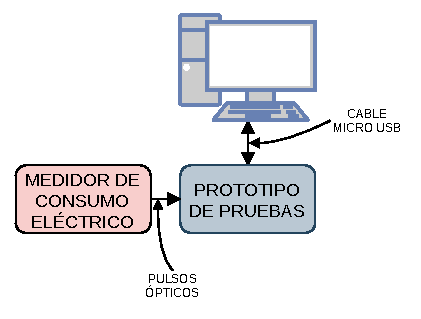
\includegraphics[scale=1.2]{./Figures/test_firmware_functional.pdf}
	\caption{Banco de pruebas para evaluar el funcionamiento del firmware.}
	\label{fig:testFunctional}
\end{figure}

Las pruebas consistieron en monitorear a través de la PC el funcionamiento de los módulos que componen la capa APP. Para esto, se añadieron instrucciones en el código fuente de estos módulos, que sirvieron para imprimir mensajes por el puerto serial. En la PC se ejecutó la utilidad idf-monitor, que es una terminal para puerto serial incluida en el ESP8266\_RTOS\_SDK. A medida que se desarrollaron los módulos, estos fueron probados individualmente verificando su correcto funcionamiento. 

Con todos los módulos funcionando individualmente, se realizó la prueba de integración de la capa APP. En la figura \ref{fig:testIDF1} se observa una captura de pantalla del idf-monitor cuando el dispositivo inicia su operación.

\begin{figure}[ht]
	\centering
	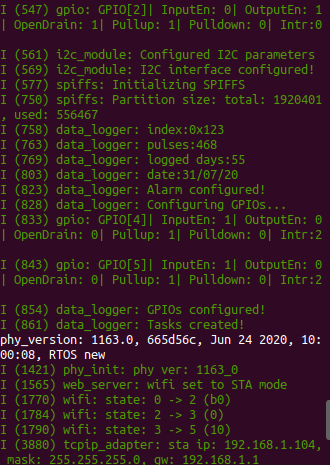
\includegraphics[scale=0.55]{./Figures/test_firmware_init.png}
	\caption{Captura de pantalla de idf-monitor cuando el dispositivo inicia.}
	\label{fig:testIDF1}
\end{figure}

Las funciones que se ejecutan en el sistema operativo del dispositivo también generaron mensajes informativos. En la captura de pantalla de la figura \ref{fig:testIDF2}, se observan los mensajes que imprimen las tareas de los módulos cuando funciona normalmente.

\begin{figure}[ht]
	\centering
	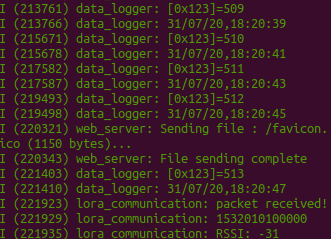
\includegraphics[scale=0.55]{./Figures/test_firmware_tasks.png}
	\caption{Captura de pantalla de idf-monitor cuando el dispositivo ejecuta sus funciones normales.}
	\label{fig:testIDF2}
\end{figure}

Con ayuda de todos los mensajes generados, además de los diagramas de flujo presentados en el capítulo \ref{Chapter3}, se pudo probar que los módulos de firmware del dispositivo funcionan correctamente.

%----------------------------------------------------------------------------------------

\section{Pruebas de la interfaz web}

Las pruebas realizadas sobre la interfaz web tuvieron la finalidad de corroborar su funcionalidad. De acuerdo a lo expuesto en el capítulo \ref{Chapter3}, el dispositivo puede ser configurado mediante el módulo WEB SERVER en dos modos de operación. Entonces, se realizaron dos tipos de pruebas distintas, una con el dispositivo como punto de acceso y la otra como estación. Para estas pruebas se utilizó una PC, un cable micro USB, un \textit{router} Wi-Fi TL-WR940N de la firme TP-Link y una \textit{laptop} con el navegador web Chrome instalado. En la figura \ref{fig:testInterface} se puede ver un diagrama del banco de pruebas montado.

\begin{figure}[ht]
	\centering
	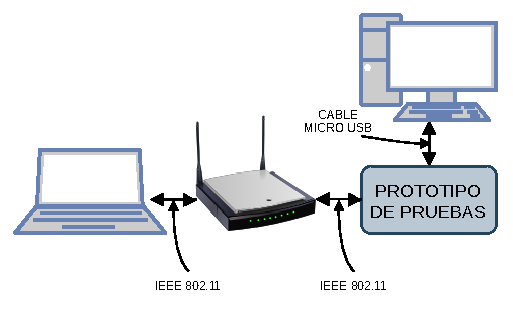
\includegraphics[scale=1.1]{./Figures/test_interface_bank.pdf}
	\caption{Banco de pruebas para verificar el funcionamiento de la interfaz web cuando el dispositivo está en modo punto de acceso.}
	\label{fig:testInterface}
\end{figure}

El primer paso fue eliminar todas las configuraciones existentes en el sistema de archivos del dispositivo, lo que provocó que al iniciar se ejecutaran las instrucciones por defecto del mismo. Por defecto el dispositivo se configura como punto de acceso. Luego, se conectó la laptop a la red Wi-Fi del dispositivo. En la figura \ref{fig:testScreenNet} se observa la red Wi-Fi generada por el dispositivo en el administrador de redes de la laptop. 

\begin{figure}[ht]
	\centering
	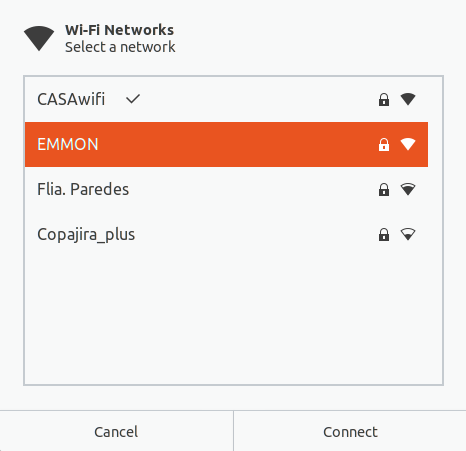
\includegraphics[scale=0.53]{./Figures/test_interface_nets.png}
	\caption{Captura de pantalla de las redes Wi-Fi disponibles en la laptop.}
	\label{fig:testScreenNet}
\end{figure}

El siguiente paso fue ingresar a la dirección de red del dispositivo mediante el navegador web de la laptop, que dio como resultado la transferencia del archivo index.html. Este archivo HTML solicitó automáticamente al dispositivo mediante el método GET todos los elementos restantes para generar la interfaz web. Para verificar que las transferencias de estos archivos se hicieran correctamente, para el lado del prototipo de pruebas se utilizó el idf-monitor y para el lado de la laptop, se hizo uso de la herramienta de depuración del navegador. En las figuras \ref{fig:testScreenBrowserDebug} y \ref{fig:testScreenIDFTransfer}, se muestran capturas de pantalla de la utilidad de depuración del navegador y la salida del idf-monitor, respectivamente.

\begin{figure}[ht]
	\centering
	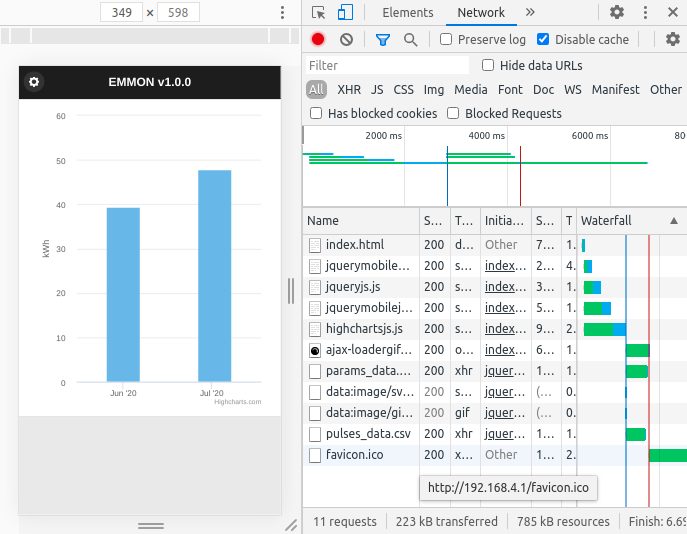
\includegraphics[scale=0.5]{./Figures/test_interface_chrome_ap.png}
	\caption{Captura de pantalla de la página principal de la interfaz web con la utilidad de depuración funcionando.}
	\label{fig:testScreenBrowserDebug}
\end{figure}

\begin{figure}[ht]
	\centering
	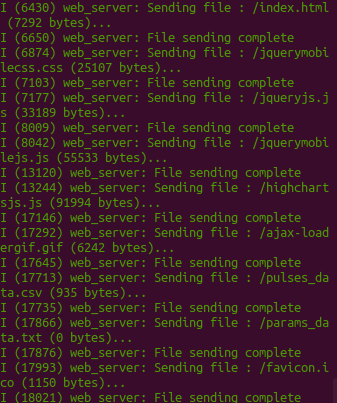
\includegraphics[scale=0.53]{./Figures/test_interface_idf_downloads.png}
	\caption{Captura de pantalla del idf-monitor después de enviar los archivos solicitados por el navegador web y el dispositivo en modo punto de acceso.}
	\label{fig:testScreenIDFTransfer}
\end{figure}

La siguiente prueba consistió en ingresar a la página de configuración de la interfaz web a través el botón ubicado en la esquina superior izquierda de la página principal. Ahí se llenó el formulario con los datos de la red Wi-Fi generada por el router, es decir, su SSID y su contraseña. Se utilizó el botón ubicado en la esquina superior derecha para enviar estos datos al prototipo de pruebas con el método POST. Con esta información el módulo WEB SERVER cambio la configuración al modo estación y pudo conectarse al router, que le proporcionó una dirección de red. Por último, la laptop también se conectó a la red del router y se utilizó el navegador web junto con la nueva dirección de red del prototipo de pruebas para solicitar los archivos de la interfaz web. En las figuras \ref{fig:testScreenWifiConf} y \ref{fig:testScreenIDFTransfer2}, se pueden observar una captura de pantalla con los campos del formulario llenados y la salida del idf-monitor, respectivamente.

\begin{figure}[ht]
	\centering
	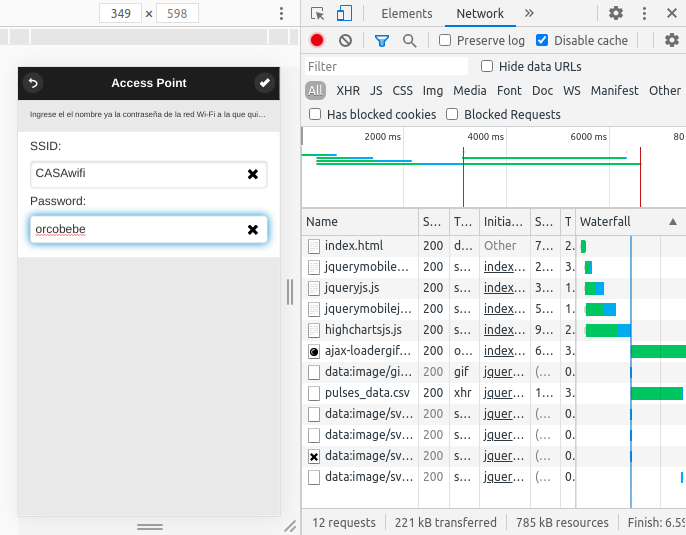
\includegraphics[scale=0.5]{./Figures/test_interface_form.png}
	\caption{Captura de pantalla de la página de configuración de la interfaz web con la utilidad de depuración funcionando.}
	\label{fig:testScreenWifiConf}
\end{figure}

\begin{figure}[ht]
	\centering
	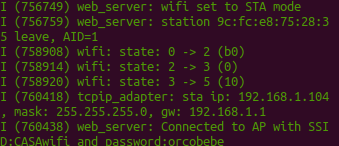
\includegraphics[scale=0.55]{./Figures/test_interface_idf.png}
	\caption{Captura de pantalla del idf-monitor después de configurar el dispositivo en modo estación con los datos enviados por la interfaz web.}
	\label{fig:testScreenIDFTransfer2}
\end{figure}

Al finalizar estas pruebas se pudo evidenciar el correcto funcionamiento de las dos páginas de la interfaz web. Asimismo, implícitamente se verificó que el módulo de firmware WEB SERVER respondía las peticiones con los métodos GET y POST según lo esperado.

%----------------------------------------------------------------------------------------
\section{Pruebas de laboratorio}

Estas pruebas tuvieron como objetivo principal utilizar instrumentación especializada para verificar el buen funcionamiento del conversor óptico-eléctrico y la fuente de alimentación. 

El propósito de la prueba del conversor óptico-eléctrico fue observar la forma de onda que genera, para implementar un algoritmo en el firmware que evitará la detección de pulsos falsos consecuencia de las características intrínsecas del LED del medidor de consumo eléctrico proporcionado por COPELECT. Para llevar a cabo esta prueba se utilizó un osciloscopio TDS2000C de la firma Tektronix, el prototipo comercial y el medidor proporcionado por COPELECT. El banco de pruebas puede observarse en el diagrama de la figura \ref{fig:testHWBankCOE}.

\begin{figure}[ht]
	\centering
	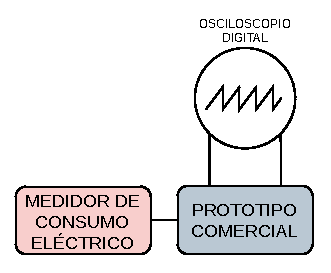
\includegraphics[scale=1.2]{./Figures/test_pulses_bank.pdf}
	\caption{Banco de pruebas para el conversor óptico-eléctrico.}
	\label{fig:testHWBankCOE}
\end{figure}

\begin{figure}[ht]
	\centering
	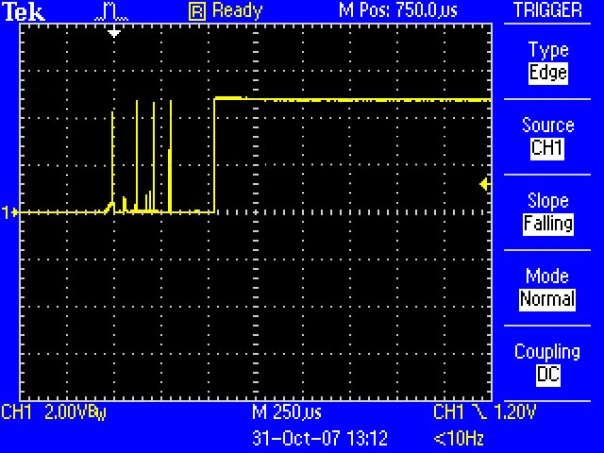
\includegraphics[scale=0.5]{./Figures/pulses_debounce.jpg}
	\caption{Salida de la pantalla del osciloscopio.}
	\label{fig:testHWPhoto}
\end{figure}

De la figura \ref{fig:testHWPhoto}, se puede observar que la forma de onda producida por el medidor tiene elementos que pueden ocasionar que el módulo DATA LOGGER registre erróneamente los pulsos y generar un reporte erróneo del consumo de energía eléctrica. Para solucionar esto, se implementó una función similar a la utilizada para detectar rebotes en los pulsadores en DATA LOGGER. Con esto se evitó en gran medida el error antes mencionado.

La prueba de la fuente de alimentación tuvo como propósito excitar este elemento con una fuente de tensión alterna, que simuló el comportamiento de la línea de alimentación cuando existen cambios en su valor nominal. Los elementos utilizados fueron una fuente de tensión alterna variable modelo 1653A de la firma BK precisión, un reóstato como carga variable y dos multímetros MUT-39 de la firma Truper. El banco de pruebas utilizado se ilustra en la figura \ref{fig:testHWBankPower}

\begin{figure}[ht]
	\centering
	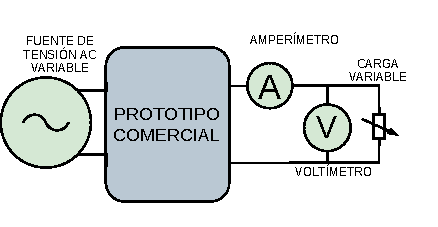
\includegraphics[scale=1.1]{./Figures/test_power_bank.pdf}
	\caption{Banco de pruebas para el conversor óptico-eléctrico.}
	\label{fig:testHWBankPower}
\end{figure}

El procedimiento consistió en establecer el nivel de tensión de entrada en un valor determinado y variar la carga conectada a la salida, para registrar los datos obtenidos del amperímetro y el voltímetro conectados en serie y paralelo, respectivamente. Los valores de tensión de entrada fueron el valor nominal de la fuente de alimentación, el valor nominal menos el 20\% y el valor nominal más el 20\%. En las tablas \ref{tab:testPower176}, \ref{tab:testPower220} y \ref{tab:testPower264}, se pueden apreciar los resultados obtenidos de estas pruebas.


\begin{table}[h]
	\centering
	\caption[Prueba de la fuente de alimentación 176 VAC]{Tabla de resultados de la prueba de la fuente de alimentación con 176 VAC.}
	\begin{tabular}{c c}    
		\toprule
		\textbf{Tensión (V)} & \textbf{Corriente (A)} \\
		\midrule
		3,27 & 0,2 \\		
		3,26 & 0,4 \\		
		3,24 & 0,6 \\
		3,21 & 0,8 \\
		3,15 & 1 \\		
		\bottomrule
		\hline
	\end{tabular}
	\label{tab:testPower176}
\end{table}

\begin{table}[h]
	\centering
	\caption[Prueba de la fuente de alimentación 220 VAC]{Tabla de resultados de la prueba de la fuente de alimentación con 220 VAC.}
	\begin{tabular}{c c}    
		\toprule
		\textbf{Tensión (V)} & \textbf{Corriente (A)} \\
		\midrule
		3,33 & 0,2 \\		
		3,32 & 0,4 \\		
		3,3 & 0,6 \\
		3,28 & 0,8 \\
		3,24 & 1 \\
		\bottomrule
		\hline
	\end{tabular}
	\label{tab:testPower220}
\end{table}

\begin{table}[h]
	\centering
	\caption[Prueba de la fuente de alimentación 264 VAC]{Tabla de resultados de la prueba de la fuente de alimentación con 264 VAC.}
	\begin{tabular}{c c}    
		\toprule
		\textbf{Tensión (V)} & \textbf{Corriente (A)} \\
		\midrule
		3,38 & 0,2 \\		
		3,36 & 0,4 \\		
		3,33 & 0,6 \\
		3,31 & 0,8 \\
		3,28 & 1 \\
		\bottomrule
		\hline
	\end{tabular}
	\label{tab:testPower264}
\end{table}

Para visualizar más fácilmente los resultados de estas pruebas y tener una perspectiva más clara sobre la variación de la tensión de salida en función de la corriente que circula por la carga, en la figura \ref{fig:testPowerGraph} se presentan gráficamente los resultados de las pruebas anteriores. La línea roja representa la prueba con 264 VAC, la línea verde la prueba con 220 VAC y la línea azul la prueba con 176 VAC.

\begin{figure}[ht]
	\centering
	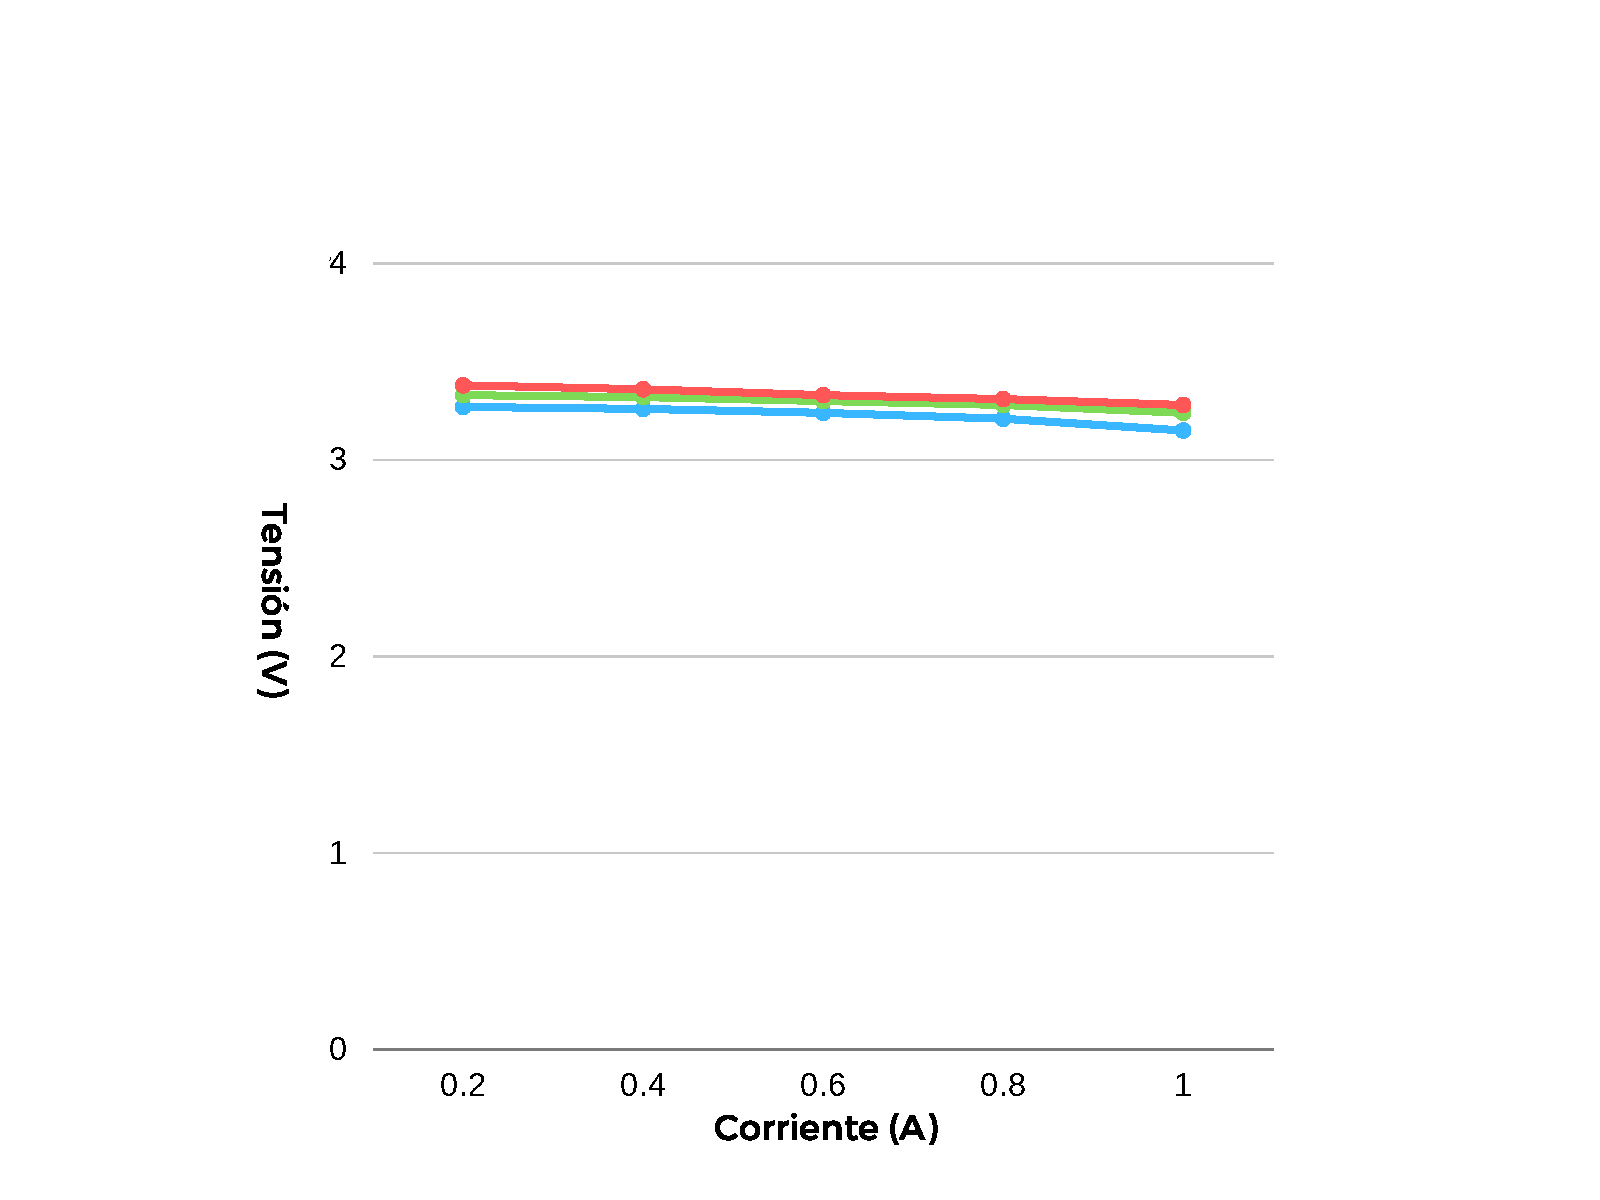
\includegraphics[scale=0.43]{./Figures/test_power_graph.pdf}
	\caption{Gráfico de líneas del comportamiento de la fuente de alimentación.}
	\label{fig:testPowerGraph}
\end{figure}

Entonces, según los valores necesarios para alimentar los componentes del prototipo comercial expuestos en la tabla \ref{tab:componentsPower} y con ayuda de las pruebas realizadas sobre la fuente de alimentación, se concluye que la fuente fue elegida correctamente para brindar los niveles de tensión y corriente adecuados cuando el valor de tensión de la línea eléctrica varíe en más o menos 20\%.

%----------------------------------------------------------------------------------------

\section{Pruebas del transceptor LoRa}

Estas pruebas fueron realizadas para determinar los parámetros adecuados del transceptor LoRa, para intercambiar información con un gateway de la misma tecnología que está ubicado en el edificio central de COPELECT. Para esto se utilizaron principalmente el prototipo comercial del dispositivo y un gateway LoRa basado en la plataforma Arduino y en el módulo LoRa PM1280. Otros elementos utilizados fueron una PC, una laptop y cables micro USB. El banco de ensayos puede observarse en la figura \ref{fig:testLoraBank}.

\begin{figure}[ht]
	\centering
	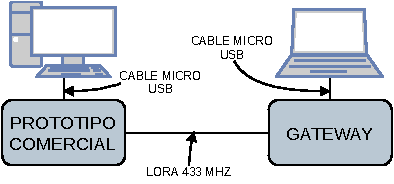
\includegraphics[scale=1]{./Figures/test_lora_bank.pdf}
	\caption{Captura de pantalla de idf-monitor después de enviar los archivos para la interfaz web.}
	\label{fig:testLoraBank}
\end{figure}

El gateway LoRa fue ubicado en la azotea del edificio central de COPELECT, que es el lugar donde debería instalarse un gateway LoRaWAN finalmente. El prototipo comercial se dispuso en el domicilio del autor, más precisamente en el mismo gabinete donde se encuentra instalado el medidor eléctrico. En la figura \ref{fig:testLoraUbi} se muestra la ubicación del gateway LoRa y el prototipo comercial.

\begin{figure}[ht]
	\centering
	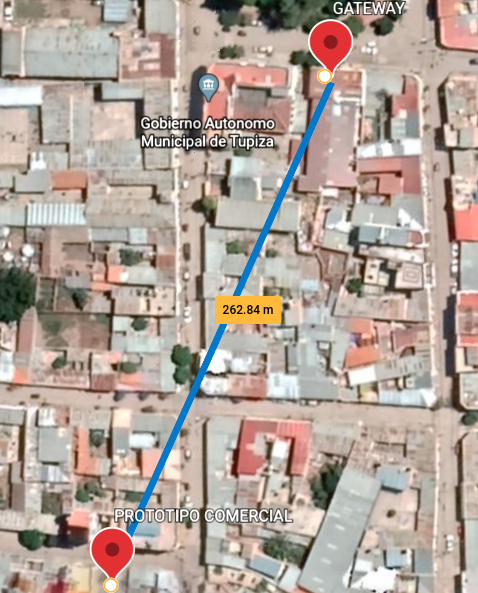
\includegraphics[scale=0.41]{./Figures/test_lora_location.png}
	\caption{Captura de pantalla de la ubicación del gateway LoRa y el prototipo comercial.}
	\label{fig:testLoraUbi}
\end{figure}

La prueba realizada consistió en el envío de un paquete con la estructura expuesta en la figura \ref{fig:loraRxPacket} por parte del prototipo comercial. Una vez que el gateway lo recibe y procesa, devuelve como respuesta un paquete con la misma estructura, que solicita una operación en el dispositivo. Con el serial monitor de Arduino instalado en la laptop se monitoreó el gateway. Mientras que para monitorear el prototipo comercial se utilizó el idf-monitor instalado en la PC. 
%Las capturas de pantalla del serial monitor y del idf-monitor, pueden observarse en las figuras \ref{fig:testLoraScreenSerial} y \ref{fig:testLoraScreenIDF}, respectivamente.
%
%\begin{figure}[ht]
%	\centering
%	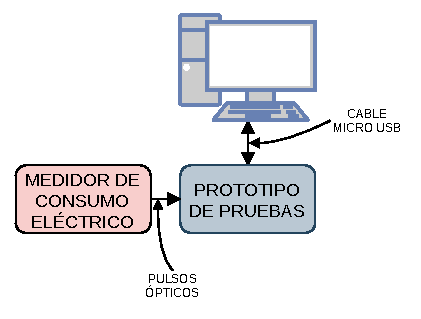
\includegraphics[scale=1.4]{./Figures/test_firmware_functional.pdf}
%	\caption{Captura de pantalla de la ubicación del gateway LoRa y el prototipo comercial.}
%	\label{fig:testLoraScreenSerial}
%\end{figure}
%
%\begin{figure}[ht]
%	\centering
%	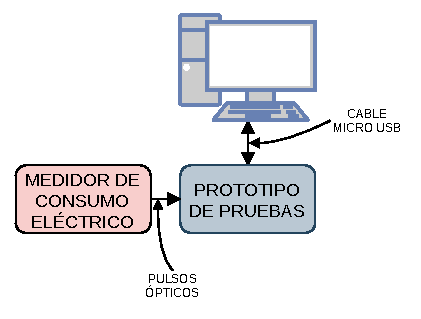
\includegraphics[scale=1.4]{./Figures/test_firmware_functional.pdf}
%	\caption{Captura de pantalla de la ubicación del gateway LoRa y el prototipo comercial.}
%	\label{fig:testLoraScreenIDF}
%\end{figure}

Se probaron distintos tipos de configuraciones para lograr una comunicación exitosa entre ambos dispositivos. Los parámetros que fueron modificados en el transceptor LoRa fueron el SF (\textit{Spreading Factor}, factor de propagación), el BW (\textit{Band Width}, ancho de banda) y el CR (\textit{Coding Rate}, tasa de codificación). En la tabla \ref{tab:testLoraTable} se muestran los valores utilizados de los parámetros antes citados.

\begin{table}[h]
	\centering
	\caption[Parámetros del transceptor LoRa]{Tabla de parámetros de configuración por software del transceptor LoRa.}
	\begin{tabular}{c c c c}    
		\toprule
		\textbf{Frecuencia (MHz)} & \textbf{BW (MHz)} & \textbf{SF} & \textbf{CR}  \\
		\midrule
		433 & 41,7 & 12 (4096 chips/symbol) & 4/5 \\		
		\bottomrule
		\hline
	\end{tabular}
	\label{tab:testLoraTable}
\end{table}

De acuerdo a los parámetros de la tabla \ref{tab:testLoraTable} se determina lo siguiente:

\begin{itemize}
	\item Entre mayor sea el BW, mayor tiempo tomará la comunicación y esto se debe a que la frecuencia es inversamente proporcional al tiempo. Sin embargo, entre menor sea la frecuencia, mayor será el alcance de transmisión esperado.
	 \item El valor de SF determina el rendimiento en la transmisión de datos, es decir, que cuanto mayor sea este valor, el dispositivo tendrá menor probabilidad de recibir datos incorrectos y tendrá mayor radio de cobertura.
	 \item El CR asegura la fiabilidad de los datos, pero cuanto mayor sea este valor más se sobrecarga el tiempo de transmisión.
\end{itemize}                                

%----------------------------------------------------------------------------------------